%!TEX encoding = IsoLatin

%% Document is article 
\documentclass[a4paper]{article}

%% ----------------------------------------------------- PACKAGES ----------------------------------------------------- %%
\usepackage{coolArticle}

%% ---------------------------------------------------- DOCUMENT ---------------------------------------------------- %%
\begin{document}

\noindent \textsc{Gallos-Montbrun} Gr�goire\\
\textsc{Faury} Louis 
	\titlebox{0.6}{Model Predictive Control}{Exercice \#1 - \textcolor{blue}{Group 2}}
	
	\vspace{10pt}
	\paragraph{} We consider the linear discrete-time LTI defined by : 
	\begin{equation}
		\begin{aligned}
			x_{i+1} &= Ax_i + Bu_i \\
			y_i &= Cx_i
		\end{aligned}
	\end{equation} 
	with : 
	\begin{equation}
		A = \begin{bmatrix} \frac{4}{3} & -\frac{2}{3} \\1 & 0\end{bmatrix}, \quad B = \begin{bmatrix} 1 \\ 0 \end{bmatrix} \quad \text{ and } \quad C = \begin{bmatrix} - \frac{2}{3} &  1\end{bmatrix}
	\end{equation}
	We can already state that the \textbf{system is controlable and observable} since the Kalman matrix and the observability matrix both are full rank : 
	\begin{equation}
		\mathcal{C} = \begin{bmatrix}  1& \frac{4}{3} \\ 0 & 1\end{bmatrix}\,, \quad \mathcal{O} = \displaystyle\begin{bmatrix}-2/3 & 1 \\ 1/9 & 4/3\end{bmatrix}
	\end{equation}
	
	\paragraph{} We consider the LQR optimization problem. Given an horizon $N$, it writes : 
	\begin{equation}
		u^* = \min_u{\left\{ V(x,u) = \sum_{i=0}^{N-1} \left[x_i^TQx_i + u_i^TRu_i\right] + x_N^TP_fx_N\right\}}
	\end{equation}
	
	with $Q=C'C + 0.001\mathbb{I}_2$, $P_f=Q$ and $R = 0.001$. 
	\section{Exercice 1}
	{
		\paragraph{} We implemented the discrete-time Riccati recursion to compute the linear feedback law that solves the LQR optimization problem. The update rules are given by, assuming a horizon $N$ : 
		\begin{equation}
			\begin{aligned}
				H_N &= P_f \\
				i=N-1\hdots 0 : \quad 
					&\left\{ \begin{aligned} K_i &= -(R+B^TH_{i+1}B)-B^TH_{i+1}A\\
									H_i &= Q+K_i^TRK_i +(A+BK_i)^TH_{i+1}(A+BK_i)
					\end{aligned}\right.
			\end{aligned}
		\end{equation}
		
		% least square ? 
	}
	
	\section{Exercice 2}
	{
	
		\begin{figure}[h!]
			\begin{minipage}{0.5\linewidth}
				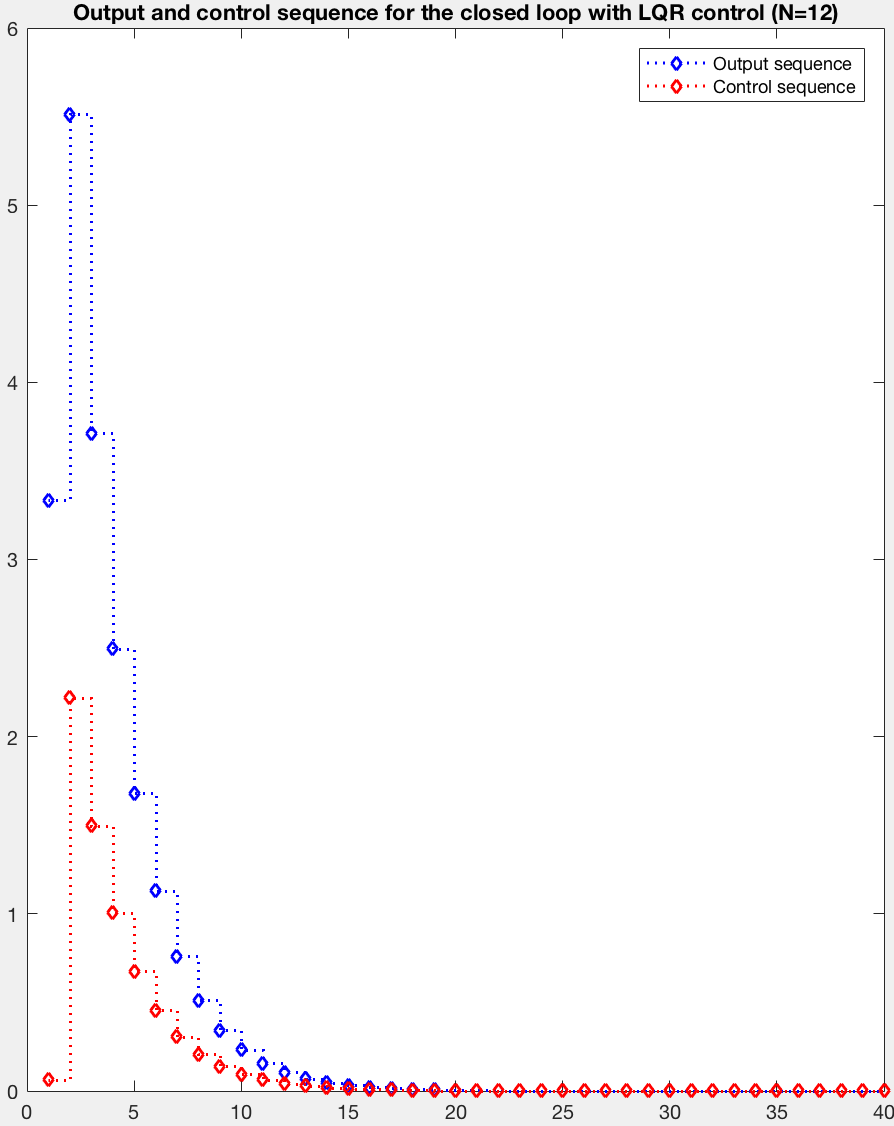
\includegraphics[width=0.9\linewidth]{traj_n12}
				\caption{Output and control sequences for N=12}
				\label{n12}
			\end{minipage}
			\begin{minipage}{0.5\linewidth}
				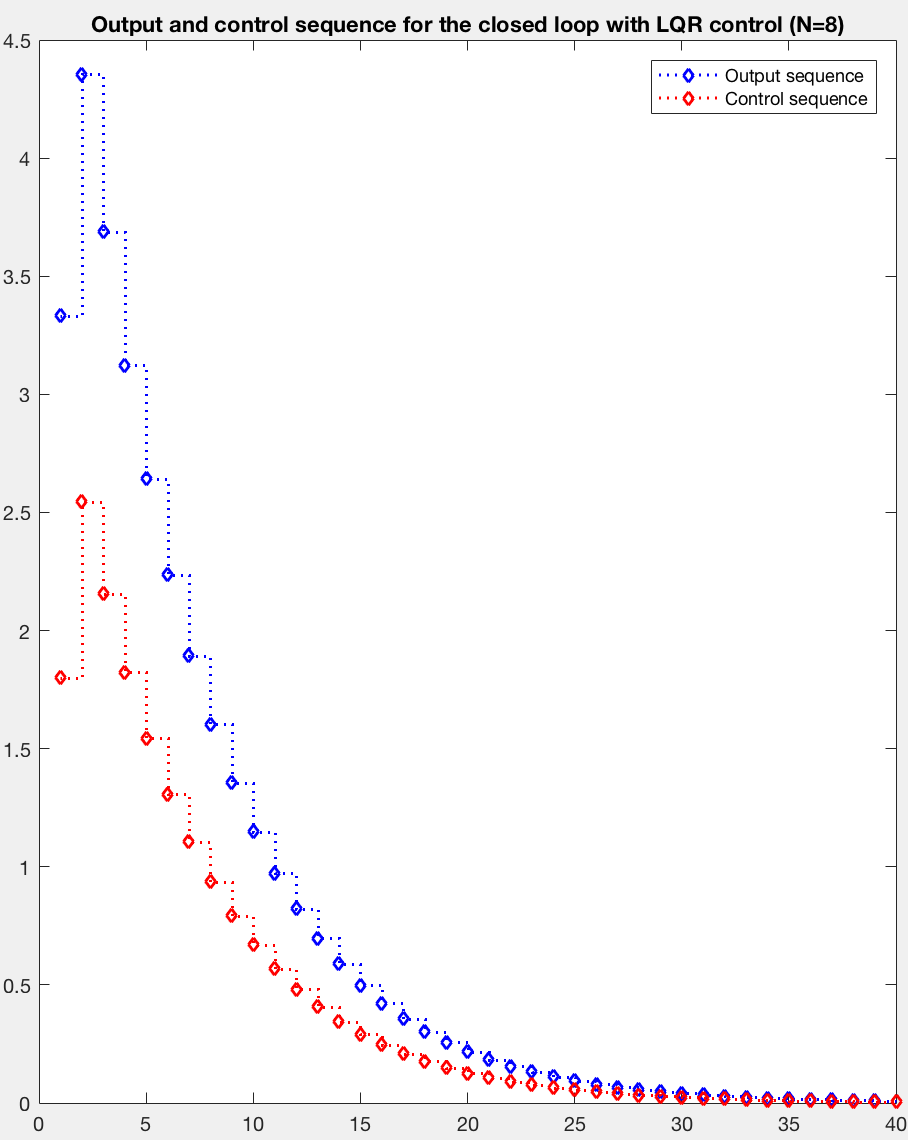
\includegraphics[width=0.9\linewidth]{traj_n8}
				\caption{Output and control sequences for N=8}	
				\label{n8}			
			\end{minipage}
		\end{figure}
		
		\paragraph{} We then implemented the LQR control in a receding horizon fashion, starting at state $x_0 = \begin{bmatrix} 10 \\ 10 \end{bmatrix}$. It is then easy to see that \fbox{\textbf{the minimum horizon length that stabilizes the system is} $\color{red} N^* = 7$}. We give a few examples of trajectories on figure (\ref{n12}) and (\ref{n8}).
		
		\paragraph{} We show the result we obtain when plotting predicted trajectories for different value of $N$ on figure (\ref{n7}) and (\ref{n10}). By increasing $N$, we see that our open-loop controller computes smoother and more realistic trajectories, as it is able to account for more futur dynamics. We see indeed that the greater the horizon is, the more the open-loop and closed-loop curve fit with one another, as future, possible unstable dynamic is accounted for. 
		
		\begin{figure}[h!]
			\begin{minipage}{0.5\linewidth}
				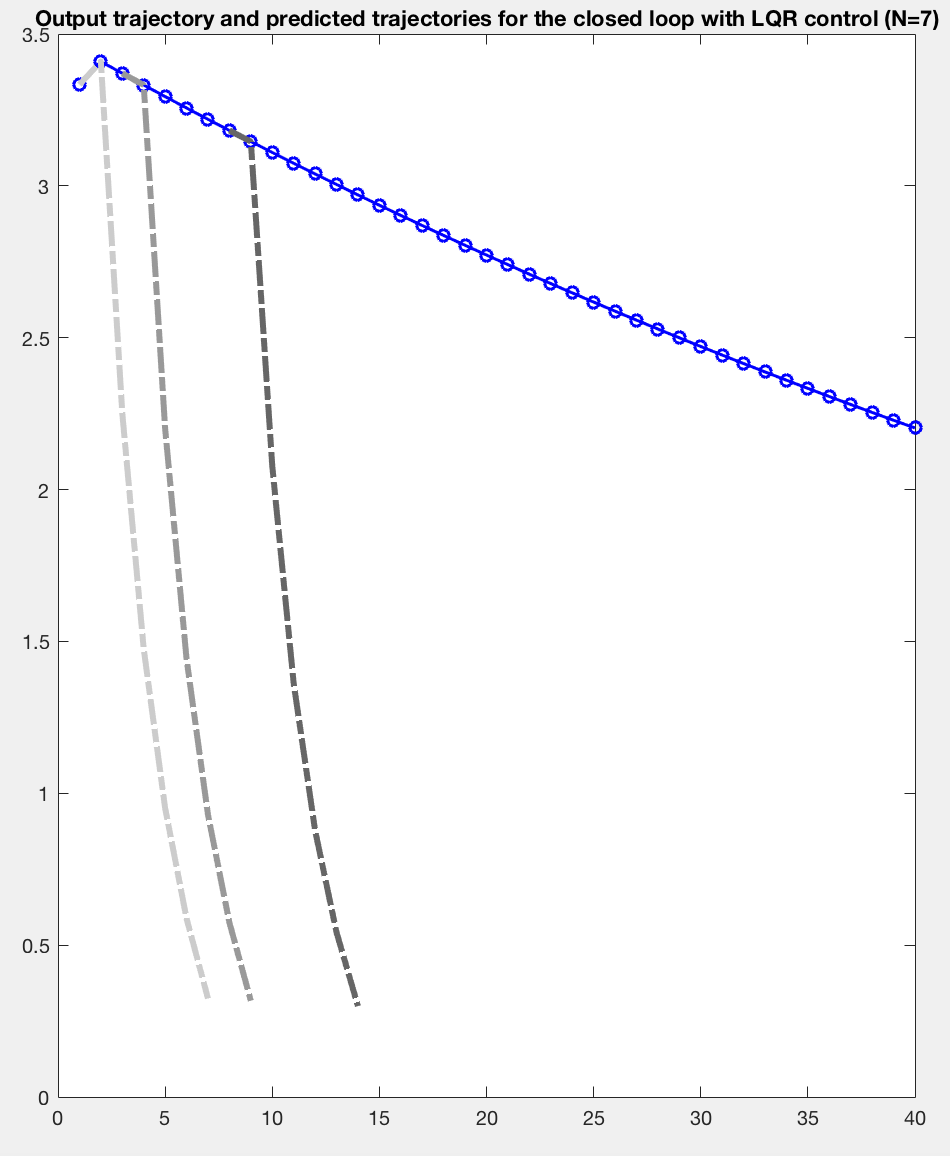
\includegraphics[width=0.9\linewidth]{pred_n7}
				\caption{Predicted and actual output trajectorie for N=7}
				\label{n7}
			\end{minipage}
			\begin{minipage}{0.5\linewidth}
				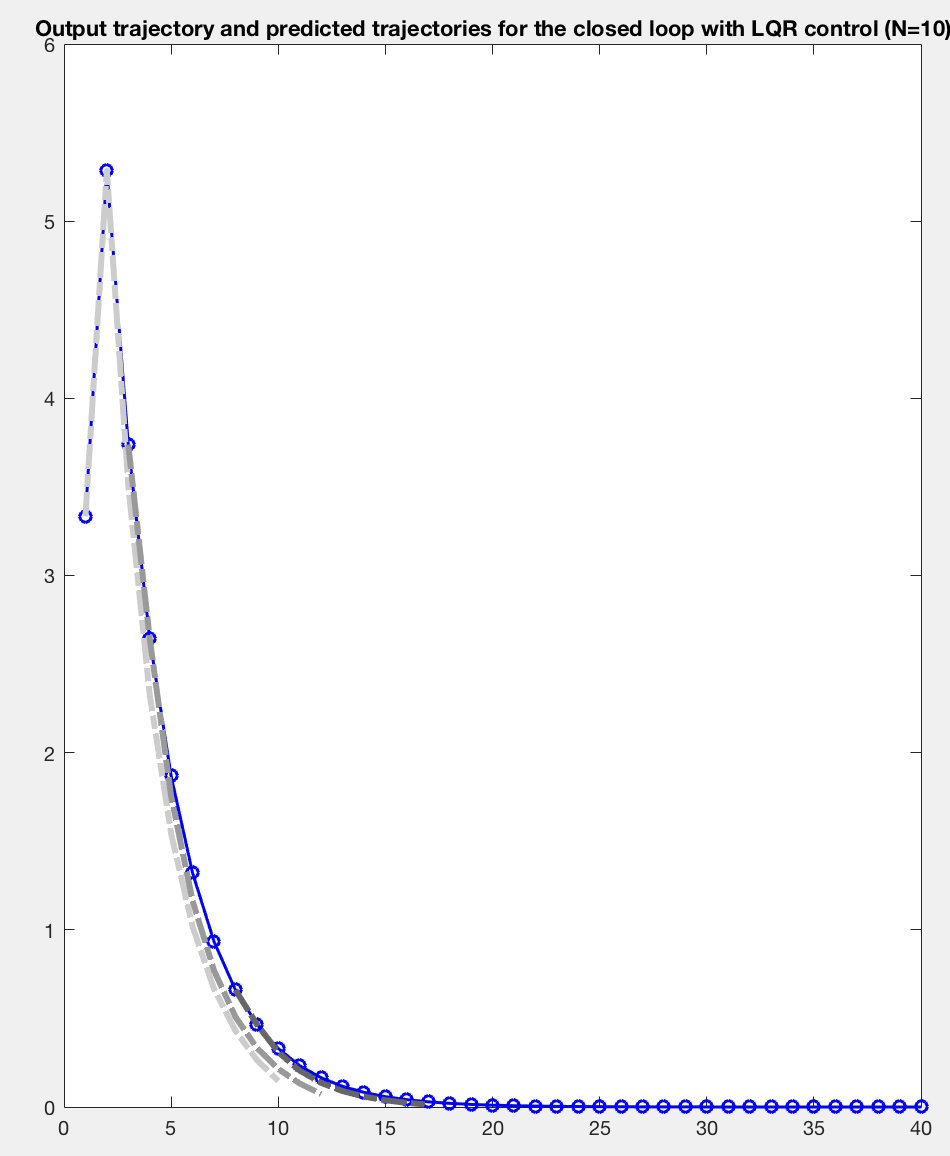
\includegraphics[width=0.9\linewidth]{pred_n10}
				\caption{Predicted and actual output trajectorie for N=10}	
				\label{n10}			
			\end{minipage}
		\end{figure}
		
		\paragraph{} Also, \emph{as illustrated in the course}, they are \fbox{no result proving that if the horizon $N^*$ stabilizes the system}, \fbox{than for any horizon $N>N^*$, the system will be stabilized}. 
	}

\end{document}